\documentclass{beamer}

\usepackage{cmap}				% To be able to copy-paste russian text from pdf
\usepackage[T2A]{fontenc}
\usepackage[utf8]{inputenc}
\usepackage[english]{babel}
\usepackage{textpos}
\usepackage{ragged2e}
\usepackage{amssymb}
\usepackage{ulem}
\usepackage{tikz}
\usepackage{pgfplots}
\usepackage{color}
\usepackage{cancel}
\usepackage{multirow}
\pgfplotsset{compat=1.17}
\usetikzlibrary{arrows,snakes,backgrounds,shapes}
\usepgfplotslibrary{groupplots,colorbrewer,dateplot,statistics}
\usepackage{animate}

\usepackage{amsfonts}
\usepackage{amsmath}
\usepackage{amssymb}
\usepackage{graphicx}
\usepackage{setspace}

\usepackage{enumitem}
\setitemize{label=\usebeamerfont*{itemize item}%
  \usebeamercolor[fg]{itemize item}
  \usebeamertemplate{itemize item}}

% remove navigation bar
\setbeamertemplate{navigation symbols}{} 

\usepackage{eurosym}
\renewcommand{\EUR}[1]{\textup{\euro}#1}

\title{Technical Notes on Interest Rates}
\author{Artem Bakulin}
\date{October 17, 2023}

\usetheme{Warsaw}
\usecolortheme{beaver}

% remove navigation bar
\setbeamertemplate{navigation symbols}{}

\setbeamertemplate{page number in head/foot}[totalframenumber] 

\newcommand{\ru}[1]{\begin{otherlanguage}{russian}#1\end{otherlanguage}}
\newcommand{\en}[1]{\begin{otherlanguage}{english}#1\end{otherlanguage}}
\newcommand{\ruen}[2]{#1 (\en{#2})}

\begin{document}



\begin{frame}
\titlepage
\end{frame}

\begin{frame}{Compound interest}
\justify
"Compound interest is the most powerful force in the universe" (attribution to Albert Einstein is wrong).

\justify
Consider a deposit at interest rate $r$ for $T$ years. Interest compounding frequency is $f$ times a year. Initial amount is $N_0$. At the end an investor will receive
\begin{align*}
N &= N_0\underbrace{\left(1 + \frac{r}{f}\right) \cdot \left(1 + \frac{r}{f}\right) \cdot ... \cdot \left(1 + \frac{r}{f}\right)}_{fT \text{terms}} = 
N_0\left(1 + \frac{r}{f}\right)^{fT}
\end{align*}

Example: a deposit of 1\,000\,000 at 12\% for 1 year with monthly compounding:
\begin{align*}
1\,000\,000 \cdot \left(1 + \frac{0.12}{12}\right)^{12} \approx 1\,126\,825
\end{align*}
\end{frame}



\begin{frame}{Common capitalization frequencies}
\centering
\begin{tabular}{l|l}
Frequency ($f$) & Name \\ \hline 
0 & Zero (no compounding) \\
1 & Annually \\
2 & Semi-annually \\
4 & Quarterly \\
12 & Monthly \\
365 & Daily \\
$\infty$ & Continuously 
\end{tabular}

\justify
Simple interest (also known as zero compounding), $f=0$:
\begin{align*}
N = N_0 (1 + rT)
\end{align*}

Continuous compounding, $f=\infty$:
\begin{align*}
N = N_0e^{rT}
\end{align*}
\end{frame}



\begin{frame}{Continuously compounded interest rate}
\justify
Suppose that we add a tiny interest to the deposit every hour, every minute, every second. Compounding frequency $f$ goes to infinity.

\begin{align*}
N &= N_0 \lim_{f \to +\infty} \left(1 + \frac{r}{f}\right)^{fT} = 
\begin{Bmatrix}x= f/r \\ f=xr \\ x \to +\infty \\ f \to +\infty\end{Bmatrix} = \\
&= N_0\lim_{x \to +\infty} \left(1 + \frac{r}{xr}\right) ^ {xrT} =
N_0{\underbrace{\left(\lim_{x \to +\infty} \left( 1 + \frac{1}{x} \right) ^ x\right)}_{e \approx 2.71828}}  ^ {rT} = \\
&= N_0e^{rT} \approx N_0(1 + rT)
\end{align*}
Continuously compounded interest rates are very uncommon in real life, but they help us make theoretical formulas a bit more concise.
\end{frame}



\begin{frame}{Compound interest  - 1}
\justify
Consider deposits of 1\,000\,000 at the interest rate of 12\% with terms of 1 and 5 years. How does terminal amount on the account depend on compounding frequency?


\begin{table}
\centering
\begin{tabular}{l|r|r|r}
Compounding frequency & $f$ & 1 year & 5 years \\ \hline
Zero & 0         & 1\,120\,000 & 1\,600\,000 \\
Annually          & 1         & 1\,120\,000 & 1\,762\,342 \\
Semi-annually     & 2         & 1\,123\,600 & 1\,790\,848 \\
Quarterly     & 4         & 1\,125\,509 & 1\,806\,111 \\
Monthly        & 12        & 1\,126\,825 & 1\,816\,697 \\
Daily         & 365       & 1\,127\,475 & 1\,821\,939 \\
Continuously        & $+\infty$ & 1\,127\,497 & 1\,822\,119
\end{tabular}
\end{table}

\justifying
The higher the interest rate and longer the term, the more important becomes compounding frequency. Daily compounding is a reasonably good  approximation of continuous compounding.
\end{frame}



\begin{frame}{Compound interest - 2}

	\centering
	\begin{tikzpicture}
		\begin{axis}[
			xlabel=\text{Time, months},
			ylabel=\text{Deposit amount},
			xmin=0,
			xmax=24.5,
			width=\textwidth,
			height=\textheight - 1.5cm,
			ymin=100,
			ymax=130,
			legend style={at={(0.01, 0.99)}, anchor=north west}
		]
	

		\addplot[const plot, samples at={0,0.1,...,60}, very thick, color=Set1-A] {100 * (1 + 0.12/4) ^ (4*3*floor(x/3)/12.0)};
		\addlegendentry{$f=4$}
	
		\addplot[const plot, samples at={0,0.5,...,60}, very thick, color=Set1-B] {100 * (1 + 0.12/12) ^ (12*floor(x)/12.0)};
		\addlegendentry{$f=12$}
		
		\addplot[domain=0:60, color=Set1-C, very thick] {100 * exp(0.12*x/12)};
		\addlegendentry{$f=+\infty$}
		\end{axis}
	\end{tikzpicture}
	\scriptsize{Growth of the deposit over time, $N_0=100$, $r=12\%$}
\end{frame}



\begin{frame}{Day count conventions}
\justify
How many years are there between March 1, 2023 and April 1, 2023?

\justify
\centering
\begin{tabular}{l|l}
Convention & Year fraction \\ \hline
ACT/365 & $31/365 \approx 0.08493$ \\
ACT/360 & $30/360 \approx 0.08611$ \\
30/360  & $30/360 \approx 0.08333$ \\
BUS/252 & $23/252 \approx 0.09127$ 
\end{tabular}

\justify
ACT --- count calendar days. 30 --- assume there are 30 days in each month. BUS --- count only business days.

\justify
Which method should you choose? Usually there is a market convention. Rule of thumb: ACT/365 in the British Commonwealth, ACT/360 in most other countries, BUS/252 in Brazil. 
\end{frame}



\begin{frame}{30/360 convention}
\justify
How many years are there between dates $D_1.M_1.Y_1$ and $D_2.M_2.Y_2$?
\begin{align*}
T = \frac{360(Y_2-Y_1) + 30(M_2-M_1) + (D_2-D_1)}{360}
\end{align*}

\justify
The 30/360 convention originated in pre-computer era, because it allows for quick mental math. It is still being used, for example, on the bond market.
\begin{itemize}
\item Backward compatibility
\item The size of interest payments does not fluctuate during the year
\end{itemize}

\vspace{\baselineskip}
\justify
* There are some variations: 30/360 Bond, 30/360 US, 30E/360, 30E/360 ISDA. They differ in handling February and 31-days months. Kudos to financial math libraries which hide these details from us!
\end{frame}



\begin{frame}{Converting between methods of compounding}
\justify
Suppose that you know a continuously compounded interest rate $r^*$, and you need a rate $r$ at frequency $f$ or vice versa. Then you can convert between conventions.
\begin{align*}
e^{r^*T} &= \left(1 + \frac{r}{f}\right)^{fT} \\
r^* &= f\ln \left(1 + \frac{r}{f}\right) \\
r &= f\left(e^{r^*/f} - 1\right)
\end{align*}

\justify
The same approach is also valid for zero rates without compounding.
\begin{align*}
e^{r^*T} &= 1+rT \\
r^* &= \frac{\ln(1+rT)}{T} \\
r &= \frac{e^{r^*T}-1}{T}
\end{align*}

\end{frame}



\begin{frame}{Present value}
\justify
\alert{Present value} of a cashflow of $N$ units of currency in $T$ years is the price which market participants would be willing to pay today to be entitled for this future cashflow.

\justify
How much USD you would be willing to pay today (present value, PV) to be entitled to receive 1\,050\,000 USD in one year (future value, FV)? Suppose that the market offers and ideal risk-free deposit at 5\% with zero compounding.

\begin{align*}
PV = \frac{FV}{1+rT} = \frac{1\,050\,000}{1 + 5\%} = 1\,000\,000
\end{align*}

\justify
Nobody will be willing to pay more than 1\,000\,000 current dollars for 1\,050\,000 future dollars. It would be more profitable to deposit current dollars at 5\%.

\justify
There is no sense in selling 1\,050\,000 future dollars cheaper than 1\,000\,000 today, because one could borrow dollars today at 5\% and pay the debt in 1 year.
\end{frame}



\begin{frame}{Discount factor}
\justify
\alert{Discount factor} for a future date $T$ is present value of a cashflow of 1 unit of a currency on date $T$. How many units of a currency one needs to posses today in order to make 1 unit of a currency by time $T$?

\justify
The answer depends on risk-free interest rate:
\begin{align*}
\delta_T &= \frac{1}{1 + rT} \quad \text{(simple interest)} \\
\delta_T &= \frac{1}{e^{r^*T}} = e^{-r^*T} \quad \text{(continuously compounded interest)}
\end{align*}

\justify
For example, suppose that risk-free interest rate is 5\%.  Discount factor for 1 year us then
\begin{align*}
\delta_1 = \frac{1}{1.05} \approx 0.9524
\end{align*}
\end{frame}



\begin{frame}{Deferred deposit}
\justify
The market offers two deposits (simple interest)
\begin{itemize}
\item Term $T_1=1$ year, interest rate $r_1=5\%$ 
\item Term $T_2=2$ years, interest rate $r_2=4\%$ 
\end{itemize}

A bank offers a  "deferred" deposit. You are obliged to deposit the cash in 1 year for 1 year. The bank is obliged to tell you the interest rate $x$ today. What would be fair rate for this deposit?

\centering
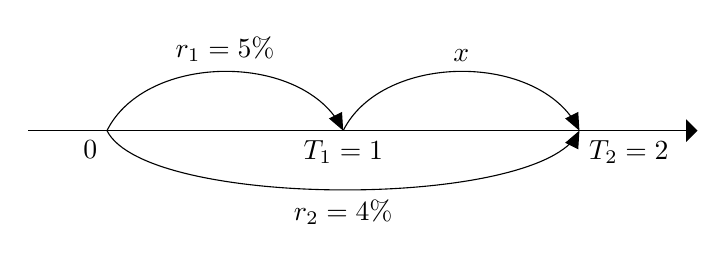
\begin{tikzpicture}
		\draw [->,>=triangle 90] (0, 0) -- (8.5, 0);

		\draw [->,>=triangle 45] (1,0) node[anchor=north east]{$0$} .. controls (1.5, 1) and (3.5, 1) .. (4,0) node[anchor=north]{$T_1=1$} node[pos=0.5,anchor=south]{$r_1=5\%$};

		\draw [->,>=triangle 45] (4,0) .. controls (4.5, 1) and (6.5, 1) .. (7,0) node[anchor=north west]{$T_2=2$} node[pos=0.5,anchor=south]{$x$};

		\draw [->,>=triangle 45] (1,0) .. controls (1.5, -1) and (6.5, -1) .. (7,0) node[pos=0.5,anchor=north]{$r_2=4\%$};
	\end{tikzpicture}
\end{frame}



\begin{frame}{Deferred deposit - 2}
\centering
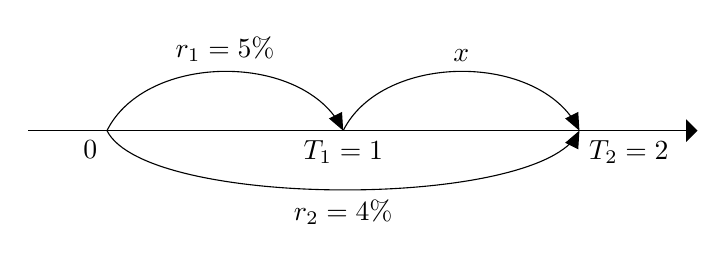
\begin{tikzpicture}
		\draw [->,>=triangle 90] (0, 0) -- (8.5, 0);

		\draw [->,>=triangle 45] (1,0) node[anchor=north east]{$0$} .. controls (1.5, 1) and (3.5, 1) .. (4,0) node[anchor=north]{$T_1=1$} node[pos=0.5,anchor=south]{$r_1=5\%$};

		\draw [->,>=triangle 45] (4,0) .. controls (4.5, 1) and (6.5, 1) .. (7,0) node[anchor=north west]{$T_2=2$} node[pos=0.5,anchor=south]{$x$};

		\draw [->,>=triangle 45] (1,0) .. controls (1.5, -1) and (6.5, -1) .. (7,0) node[pos=0.5,anchor=north]{$r_2=4\%$};
	\end{tikzpicture}
	
\justifying
The should be no difference between a longer deposit and a chain of two shorter deposits.
\begin{align*}
(1 + r_1T_1)\Big(1+x(T_2-T_1)\Big) = 1 + r_2T_2
\end{align*}
\begin{align*}
x = \frac{\dfrac{1+r_2T_2}{1+r_1T_1} - 1}{T_2-T_1} = \frac{\dfrac{1 + 0.04 \cdot 2}{1 + 0.05} - 1}{2-1} \approx 2.86\%
\end{align*}

At any other "deferred" rate $x$ the deferred deposit would be unfavorable for the bank or for clients.
\end{frame}



\begin{frame}{Continuous compounding}
\justify
Convert simple interest rate into continuously compounded rates:
\begin{align*}
r_1^* &= \frac{\ln(1+r_1T_1)}{T_1} = \frac{\ln 1.05}{1} \approx 4.879\% \\
r_2^* &= \frac{\ln(1+r_2T_2)}{T_2} = \frac{\ln 1.08}{2} \approx 3.848\%
\end{align*}

\centering
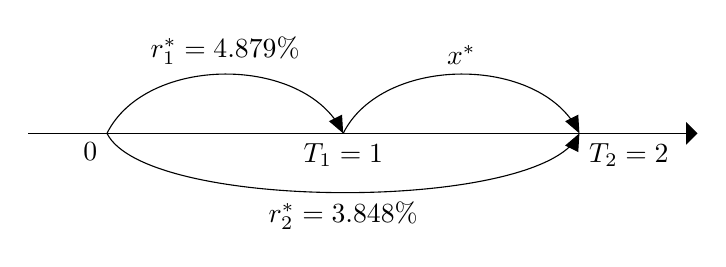
\begin{tikzpicture}
		\draw [->,>=triangle 90] (0, 0) -- (8.5, 0);

		\draw [->,>=triangle 45] (1,0) node[anchor=north east]{$0$} .. controls (1.5, 1) and (3.5, 1) .. (4,0) node[anchor=north]{$T_1=1$} node[pos=0.5,anchor=south]{$r_1^*=4.879\%$};

		\draw [->,>=triangle 45] (4,0) .. controls (4.5, 1) and (6.5, 1) .. (7,0) node[anchor=north west]{$T_2=2$} node[pos=0.5,anchor=south]{$x^*$};

		\draw [->,>=triangle 45] (1,0) .. controls (1.5, -1) and (6.5, -1) .. (7,0) node[pos=0.5,anchor=north]{$r_2^*=3.848\%$};
	\end{tikzpicture}
\end{frame}



\begin{frame}{Continuous compounding - 2}
\centering
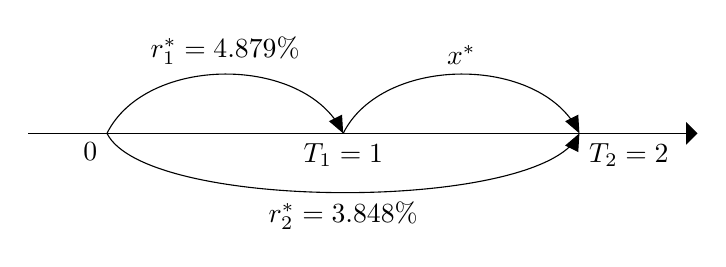
\begin{tikzpicture}
		\draw [->,>=triangle 90] (0, 0) -- (8.5, 0);

		\draw [->,>=triangle 45] (1,0) node[anchor=north east]{$0$} .. controls (1.5, 1) and (3.5, 1) .. (4,0) node[anchor=north]{$T_1=1$} node[pos=0.5,anchor=south]{$r_1^*=4.879\%$};

		\draw [->,>=triangle 45] (4,0) .. controls (4.5, 1) and (6.5, 1) .. (7,0) node[anchor=north west]{$T_2=2$} node[pos=0.5,anchor=south]{$x^*$};

		\draw [->,>=triangle 45] (1,0) .. controls (1.5, -1) and (6.5, -1) .. (7,0) node[pos=0.5,anchor=north]{$r_2^*=3.848\%$};
	\end{tikzpicture}

\justifying
There should be no difference between a 2 year deposit and a combination of two shorter deposits.
\begin{align*}
e^{r_1^*T_1}e^{x^*(T_2-T_1)} = e^{r_2^*T_2}
\end{align*}
\begin{align*}
x^* = \frac{r_2^*T_2-r_1^*T_1}{T_2-T_1} = \frac{3.848\%\cdot2 - 4.879\%}{2 - 1} \approx 2.817\%
\end{align*}

Covert continuously compounded rate back into simple interest rate:
\begin{align*}
x = \frac{e^{x^*(T_2-T_1)} - 1}{T_2 - T_1} = e^{0.02817} - 1 \approx 2.86\% 
\end{align*}
\end{frame}



\begin{frame}{Continuous compounding - 3}
\justify
People are willing to invest $100$ dollars in order to receive $105$ in one year. This is observable reality. We can interpret this as "simple" interest rate 5\%, as continuously compounded interest rate 4.879\%, as discount factor of 0.9524. These are all equivalent views (using different units of measurement) on one and the same situation.

\justify 
Depending on the context it may be more convenient to prefer one abstraction over the other. Human beings like simple interest. Continuously compounded rates simplify mathematics and source code. Discount factors help in case we know future cashflows and need to know their value in todays money.
\end{frame}


\end{document}